\documentclass{beamer}

\usepackage{graphicx}


\begin{document}
%====================================================== %
\begin{frame}
\frametitle{Binary Integer Programming}
\large
\begin{figure}
\centering
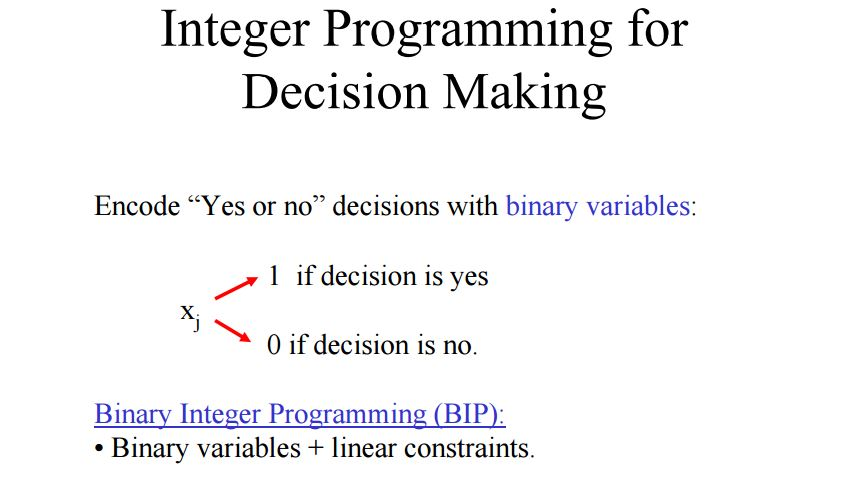
\includegraphics[width=1.1\linewidth]{calaircraft1}
\end{figure}
\end{frame}
%====================================================== %
\begin{frame}
	\frametitle{Binary Integer Programming}
	\large
	\begin{figure}
		\centering
		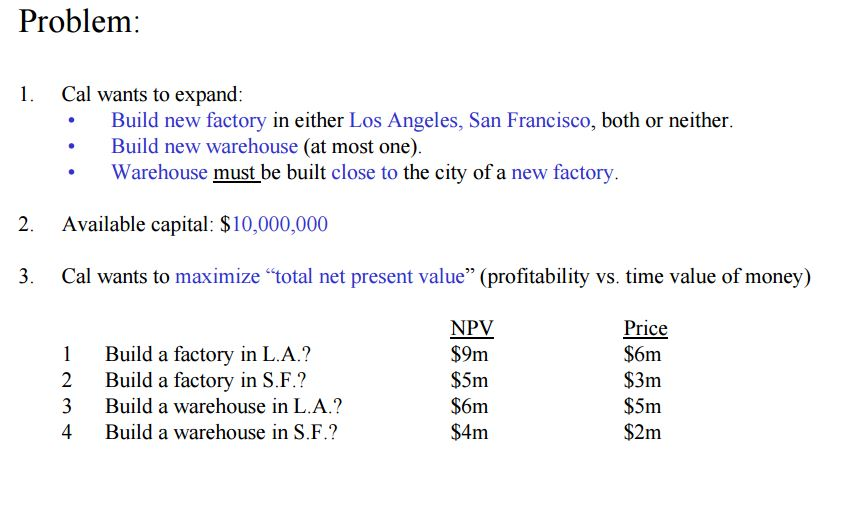
\includegraphics[width=1.1\linewidth]{calaircraft2}
	\end{figure}
\end{frame}
%====================================================== %
\begin{frame}
	\frametitle{Binary Integer Programming}
	\large
	\begin{figure}
		\centering
		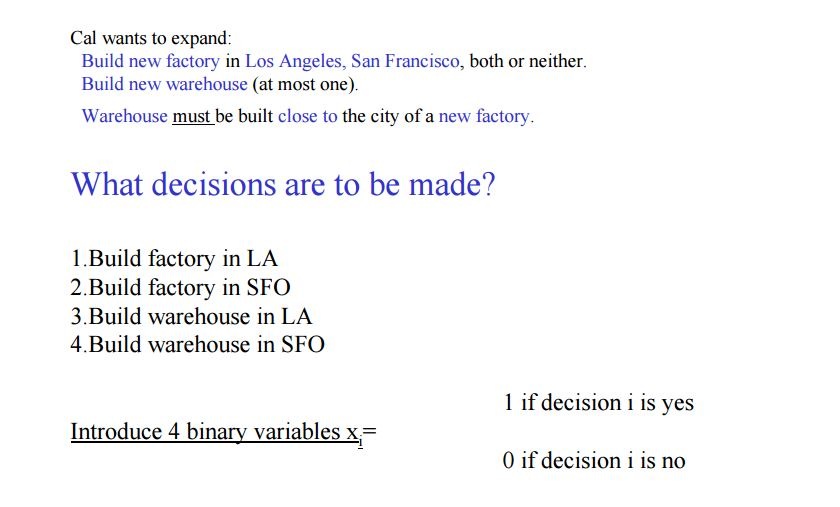
\includegraphics[width=1.1\linewidth]{calaircraft3}
	\end{figure}
\end{frame}
%====================================================== %
\begin{frame}
	\frametitle{Binary Integer Programming}
	\large
	\begin{figure}
		\centering
		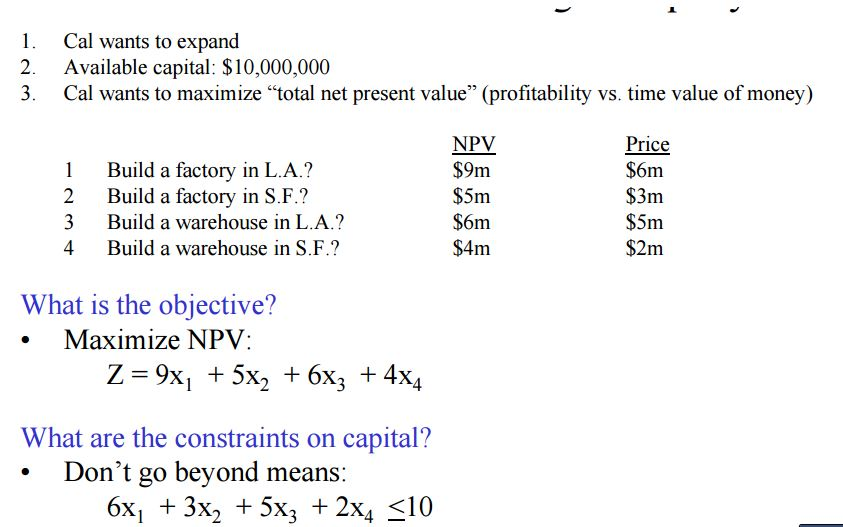
\includegraphics[width=1.1\linewidth]{calaircraft4}
	\end{figure}
\end{frame}
%====================================================== %
\begin{frame}
	\frametitle{Binary Integer Programming}
	\large
	\begin{figure}
		\centering
		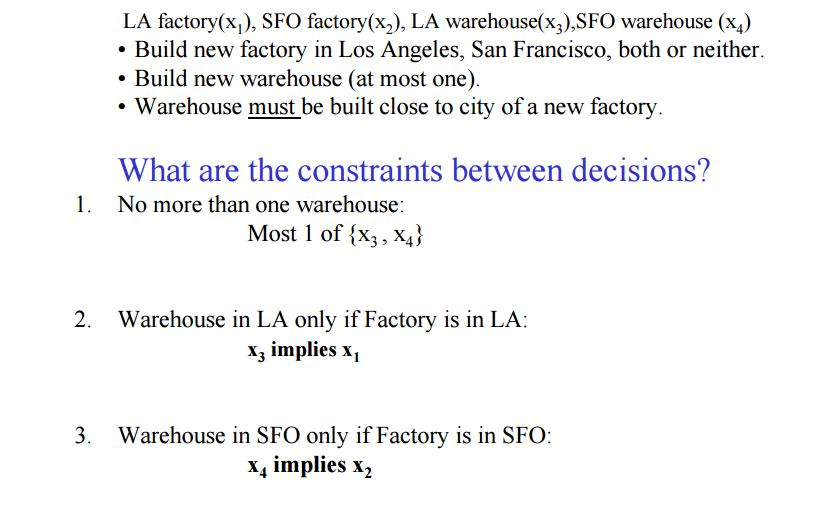
\includegraphics[width=1.1\linewidth]{calaircraft5}
	\end{figure}
\end{frame}
%====================================================== %
\begin{frame}
	\frametitle{Binary Integer Programming}
	\large
	\begin{figure}
		\centering
		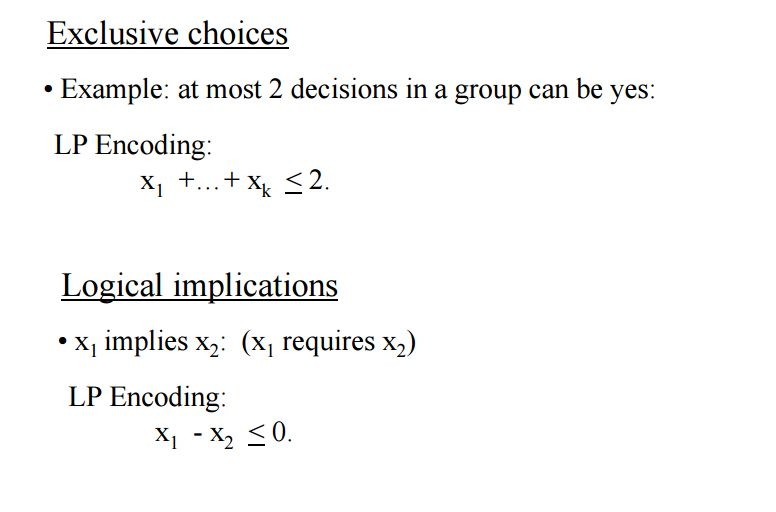
\includegraphics[width=1.1\linewidth]{calaircraft6}
	\end{figure}
\end{frame}
%====================================================== %
\begin{frame}
	\frametitle{Binary Integer Programming}
	\large
	\begin{figure}
		\centering
		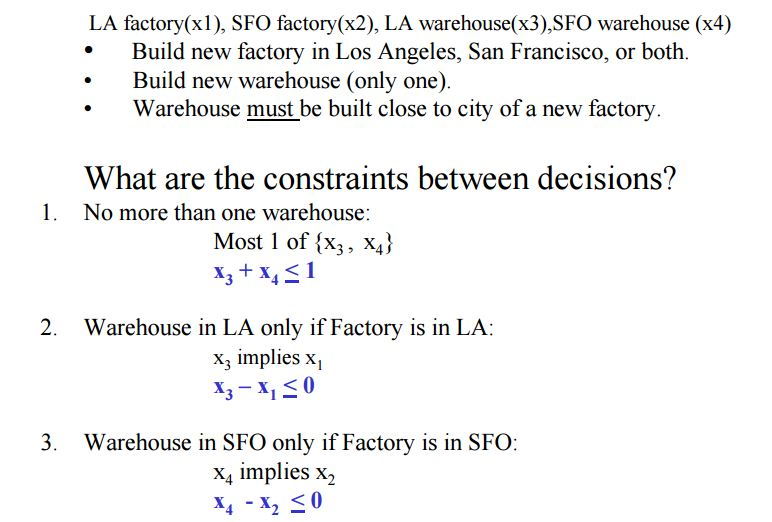
\includegraphics[width=1.1\linewidth]{calaircraft7}
	\end{figure}
\end{frame}
%====================================================== %
\begin{frame}
	\frametitle{Binary Integer Programming}
	\large
	\begin{figure}
		\centering
		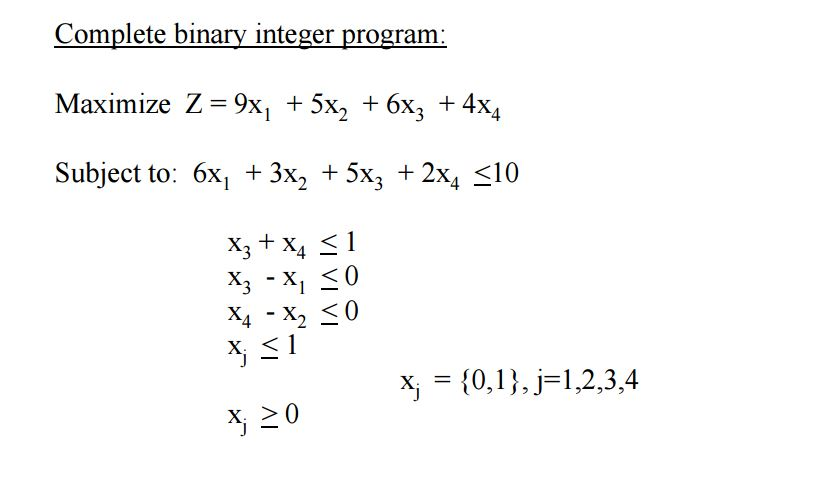
\includegraphics[width=1.1\linewidth]{calaircraft8}
	\end{figure}
\end{frame}
%====================================================== %
\begin{frame}
\frametitle{Binary Integer Programming}
\Large
\noindent\textbf{Review}
\begin{itemize}
	\item Be able to state a program for a BIP problme with the appropriate set of constraints (i.e. be able to state a problem just like the previous slide).
	\item Remember to state what $x_1$,$x_2$ etc mean.
\end{itemize}
\end{frame}
\end{document}
